\subsubsection{Stony Brook University}  
\paragraph{Ion Back Flow} A TPC prototype has been constructed and a sophisticated test-beam setup established. We purchased picoammeter from PicoLogic in Zagreb/Croatia which is a unique device that allows to measure very small currents at high potential. The floating current measurements can be performed at potentials much larger than 5 kV, ideally suited for IBF measurements in a TPC.

The TPC prototype has been equipped with a real size readout module, based on a quadruple-GEM stack similar to the ALICE-TPC readout and zig-zag pad readout structure. The prototype has been exposed to the 120 GeV protons at the Fermilab Test Beam Facility (FTBF) to establish the working parameters of the TPC. We have analyzed the data obtained from the test-beam campaign and verified the performance parameter of the prototype. The resolution has been obtained by measuring with a drift-length of 40 cm at B = 0 T and extrapolated to the magnetic field with the Babar magnet at B = 1.4 T with \[\sigma^2_{total}=\sigma^2_{int}+\frac{D^2_TL}{N_{eff}}+\sigma^2_{sc}\]
with $\sigma_{int}=\sigma(z=0)$: intrinsic resolution, $D_T$: diffusion constant, $L$: drift length, $N_{eff}$: effective number of electrons leading to the readout signal and $\sigma_{sc}$: smearing due to space charge distortions. The smearing due to space charge distortions can be neglected at the test-beam. The measurement/extrapolation principle can be taken from Fig.~\ref{fig:measPrinc}.
\begin{figure}
    \centering
    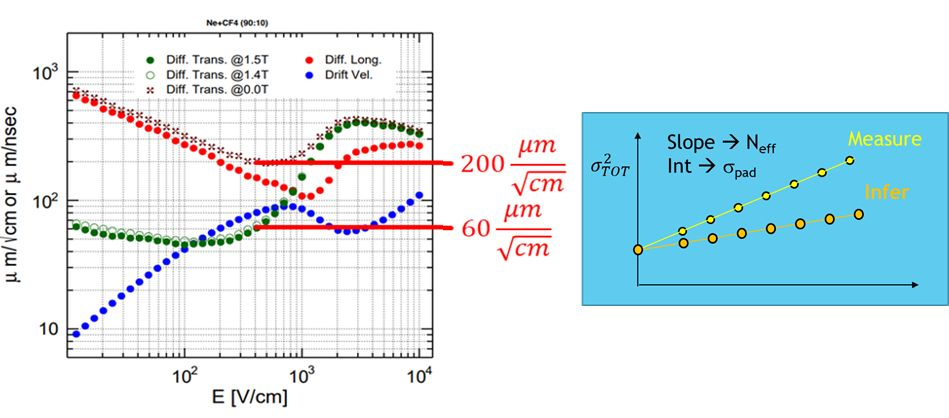
\includegraphics[width=\columnwidth]{SBU_plots/TPCresolutionPrinciple.jpg}
    \caption{\label{fig:measPrinc}Principle for the determination of space point resolution at B = 0 T and extrapolation to B = 1.4 T.}
\end{figure}
The results for this procedure are shown in Fig.~\ref{fig:TPCres}.
\begin{figure}
    \centering
    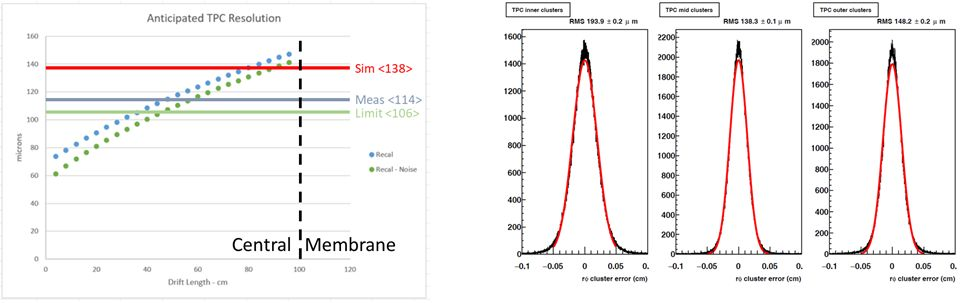
\includegraphics[width=\columnwidth]{SBU_plots/TPCresolution.jpg}
    \caption{\label{fig:TPCres}Comparison of measured (left) and simulated (right) space point resolution.}
\end{figure}

\paragraph{Mirror coating} We have continued to install components of the electron-/ion-gun for the evaporation of thin layer structures on mirror surfaces. The installation is running smoothly and undergraduate students are gaining experience in handling the sensitive equipment under the supervision of senior personnel. The installation process also helps in understanding the equipment and in preparing the start-up procedure of operation.

\paragraph{Meta-materials}
We have started evaluating procedures of transformation optics with which one can obtain properties of materials that allow to modify the Cherenkov angles but maintaining the momentum reach for high momentum particles. Based on the dispersion relation (from \cite{Vginis:2014})
\[\frac{k_x^2}{f'^2(x)}+\frac{k_y^2}{g'^2(y)}+\frac{k_z^2}{h'^2(z)}=\epsilon_b\frac{\omega^2}{c^2}.
\]
and substituting $f'(x)=F~(=\frac{\partial x}{\partial x'}),~g'(y)=G~(=\frac{\partial y}{\partial y'}),~h'(z)=H~(=\frac{\partial z}{\partial z'})$ we were able to reproduce the simulated results obtained in \cite{Vginis:2014}, Figs.~1 a) and b). These reproduced results can be seen in Figs.~\ref{fig:phiVsF}, \ref{fig:phiVsG}.

\begin{figure}
    \centering
    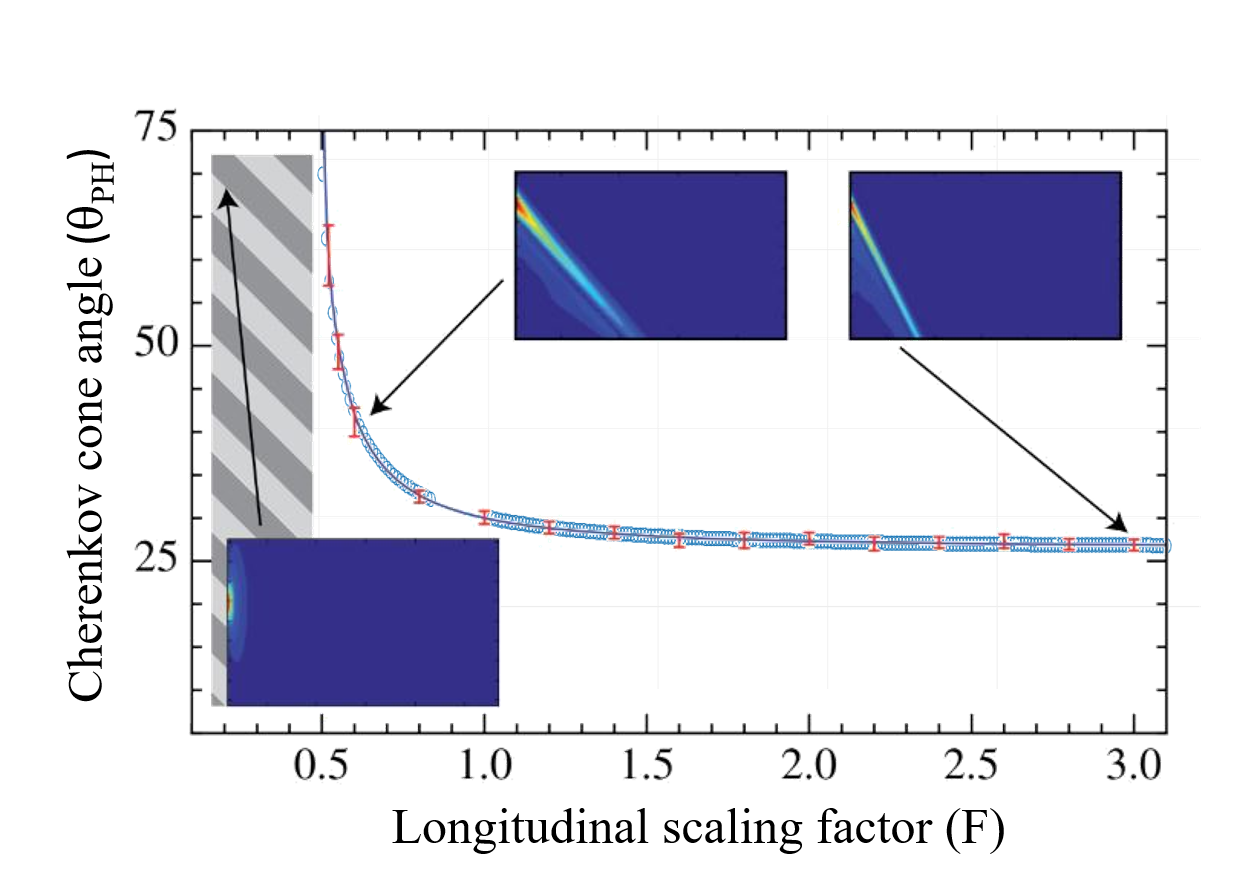
\includegraphics[width=0.8\columnwidth]{SBU_plots/phiVsFoverlayed.png}
    \caption{\label{fig:phiVsF}Data reproduction (open blue circles) based on the calculations obtained from the transformation optics overlaid on \cite{Vginis:2014} Fig.~1a).}
%\end{figure}
%\begin{figure}
%    \centering
    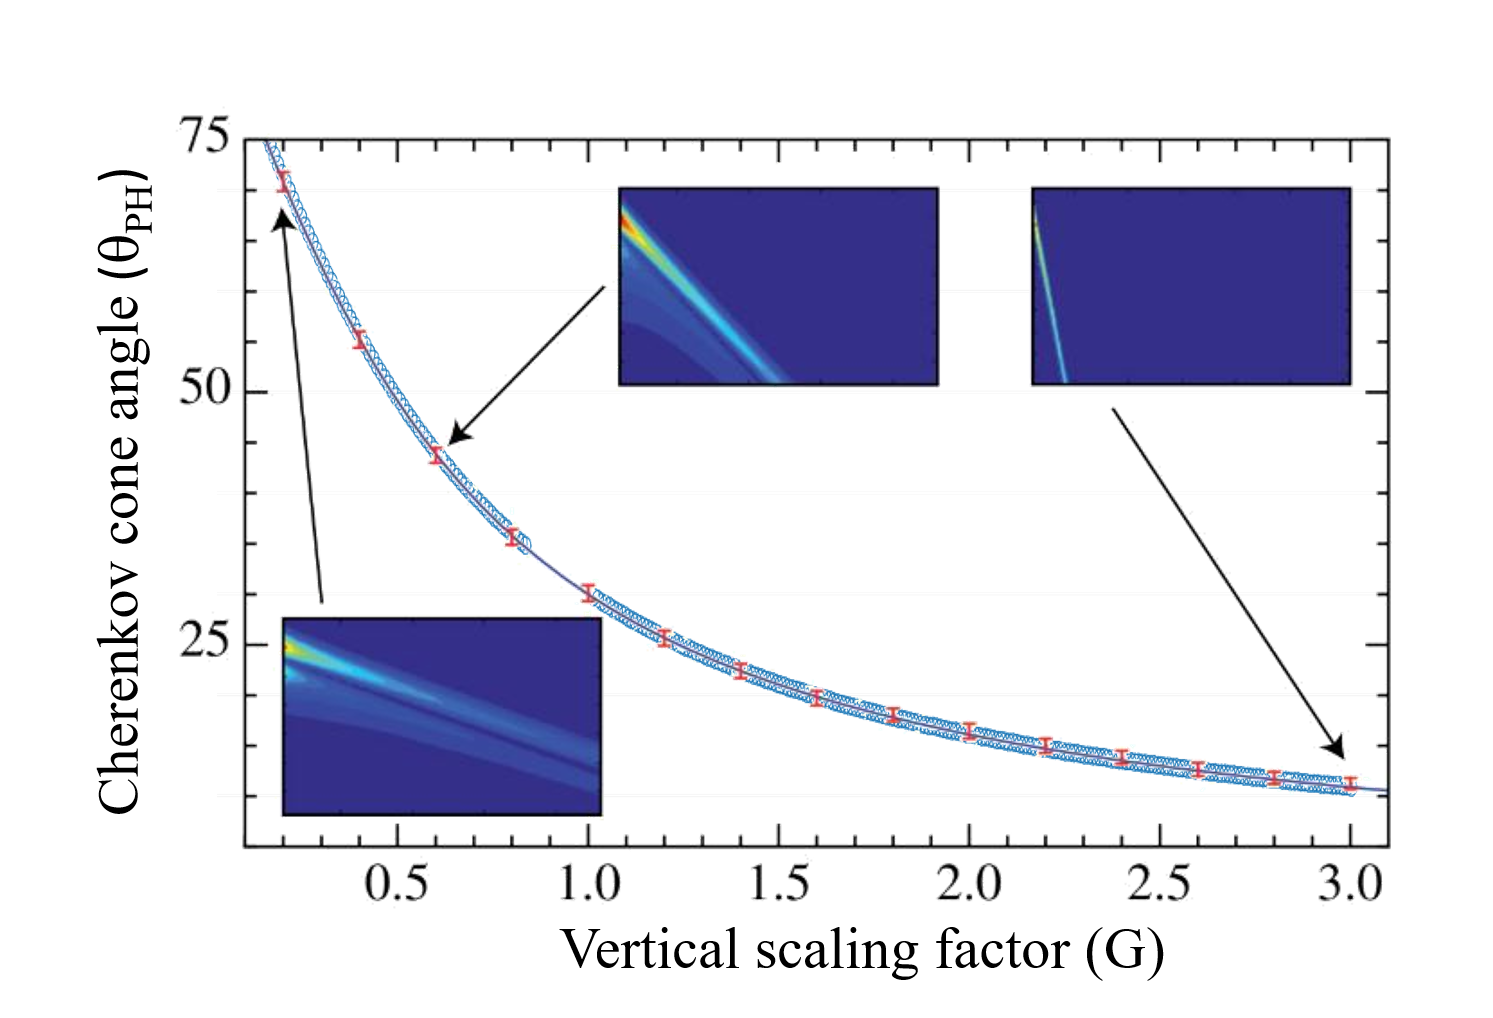
\includegraphics[width=0.8\columnwidth]{SBU_plots/phiVsGoverlayed.png}
    \caption{\label{fig:phiVsG}Data reproduction (open blue circles) based on the calculations obtained from the transformation optics overlaid on \cite{Vginis:2014} Fig.~1b).}
\end{figure}